%%%%%%%%%%%%
%
% $Autor: Sudeshna $
% $Datum: 2019-03-05 08:03:15Z $
% $Pfad: TemplateSensor $
% $Version: 4250 $
% !TeX spellcheck = en_GB/de_DE
% !TeX encoding = utf8
% !TeX root = filename 
% !TeX TXS-program:bibliography = txs:///biber
%
%%%%%%%%%%%%

% Structure
\chapter{Domain System/Complete System}
\section{Description}
	The \texttt{Arduino Nano 33 BLE Sense} is a compact and low-power board ideal for IoT and AI applications, especially when space is a constraint. Its small size (\(45mm \times 18mm\)) and efficient power usage make it perfect for projects that require long battery life, operating at \(3.3V\). This board comes with a variety of embedded sensors, making it versatile for a range of applications.\cite{Gyroplace:2023} Below is a brief summary of the features on the board:
	
	\begin{itemize}
		\item \textbf{LEDs}: The board features three different LEDs for various purposes:
		\begin{itemize}
			\item \textbf{RGB Programmable LED}: Allows you to program different colors and effects for visual feedback.
			\item \textbf{Built-in Orange Programmable LED}: Can be used for status indication or customized signals.
			\item \textbf{Power LED}: Indicates that the board is powered on.
		\end{itemize}
		\item \textbf{Processor}: The board is powered by the \texttt{nRF52840} processor, a 32-bit ARM® Cortex™-M4 CPU running at 64 MHz, which is more powerful than many other Arduino boards, allowing it to handle more complex computations or real-time data processing.
		
		\item \textbf{USB-C Port}: The \texttt{Arduino Nano 33 BLE Sense} features a \textbf{USB-C port} for power and data transfer. This modern, reversible connector provides a reliable connection for both programming the board and powering it.
		
		\item \textbf{Power Button}: The board includes a \textbf{power button}, allowing you to manually power on or off the device without needing to disconnect it from the power source. This is useful for battery-powered projects, where conserving power or resetting the device is necessary.
	\end{itemize}
	
	The \texttt{Arduino Nano 33 BLE Sense} is ideal for low-power, compact devices that require real-time environmental sensing, motion tracking, or interactive capabilities, all within a small, portable form factor.\cite{Passaro:2017}
	

\section{Design}

\begin{figure}[H]\centering
	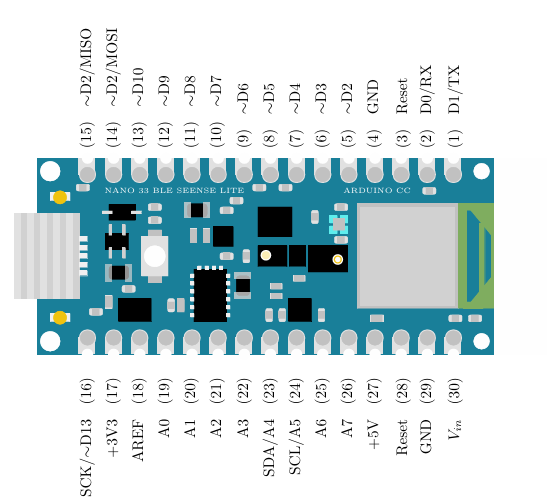
\includegraphics[width=0.8\textwidth]{Images/Sensor Actor/Pin_Assignment_of_Ardruino33BLEsense} 
	\caption{\textbf{Pin Assignment of Arduino Nano 33 BLE Sense}}
	\label{fig:Pin_assignment_of_Arduino_Nano_33_BLE_Sense} 
\end{figure}
\begin{figure}[H]\centering
	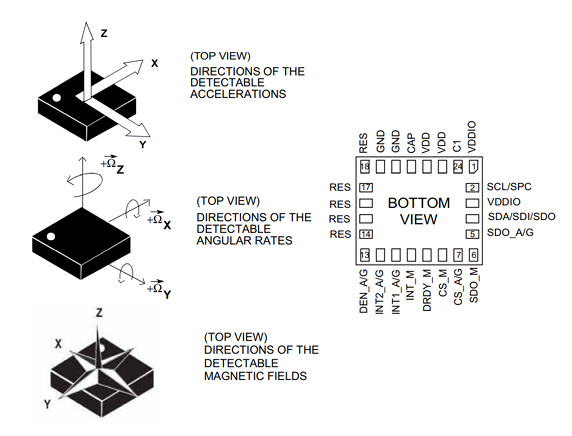
\includegraphics[width=0.8\textwidth]{Images/Sensor Actor/pin_connection_lsm9ds1} 
	\caption{\textbf{Pin Assignment of LSM9DS1}}
	\label{fig:Pin_assignment_of_Arduino_Nano_33_BLE_Sense} 
\end{figure}
\begin{figure}[H]\centering
	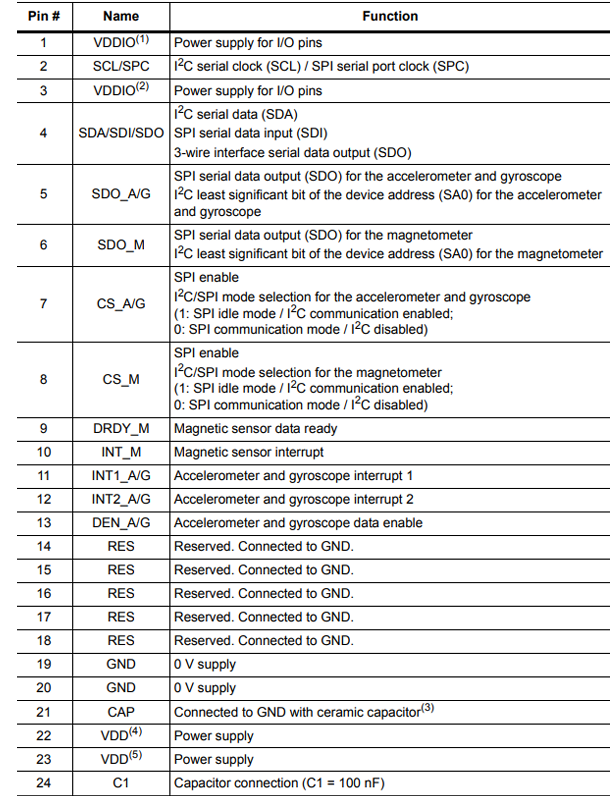
\includegraphics[width=0.8\textwidth]{Images/Sensor Actor/pin_description_lsm9ds1} 
	\caption{\textbf{Pin Description of LSM9DS1}}
	\label{fig:Pin_assignment_of_Arduino_Nano_33_BLE_Sense} 
\end{figure}
\section{Hardware Interface}

	The Arduino Nano 33 BLE Sense is a small and powerful development board featuring various hardware interfaces for communication, control, and interaction. The following sections describe the available interfaces in detail:
	
	\subsection*{1. Power and Input/Output Pins}
	
	\begin{itemize}
		\item \textbf{Power Pin}: The board operates on 3.3V, which is the nominal voltage for most sensors on the board. The power input can be supplied either through the \textbf{USB-C} port or via the \textbf{VIN} pin (which can take an input voltage of 5V to 12V).
		
		\item \textbf{GND Pins}: The board provides multiple ground (GND) pins, which are essential for completing the electrical circuit when connecting external devices and sensors.
		
		\item \textbf{Digital I/O Pins}: The Arduino Nano 33 BLE Sense features 14 digital I/O pins, out of which 12 can be used as PWM (Pulse Width Modulation) outputs. These pins are capable of reading and writing digital signals, used to control LEDs, motors, or other digital devices.
		
		\item \textbf{Analog Input Pins}: There are 8 analog input pins (A0 to A7), which are used to measure analog voltages in the range of 0 to 3.3V, useful for connecting sensors such as potentiometers, light sensors, and others that output analog signals.
		
		\item \textbf{3.3V and 5V Output Pins}: These pins allow you to supply power to external devices. The 3.3V pin is useful for low-voltage components, while the 5V pin can be used for higher voltage devices.
		
		\item \textbf{Reset Pin}: The Reset pin is used to restart the microcontroller, typically used for debugging or reinitializing the device during a project.
	\end{itemize}
	
	\subsection*{2. USB-C Interface}
	\begin{itemize}
		\item \textbf{USB-C Port}: The \texttt{Arduino Nano 33 BLE Sense} features a modern USB-C port that serves dual purposes:
		\begin{itemize}
			\item \textbf{Programming Interface}: The USB-C connection allows you to upload your sketches (code) to the board via the Arduino IDE.
			\item \textbf{Powering the Board}: The USB-C port provides a reliable power source to the board, typically at 5V, which is regulated down to 3.3V for the operation of the onboard sensors and components.
		\end{itemize}
	\end{itemize}
	
	\subsection*{3. Communication Interfaces}
	
	\begin{itemize}
		\item \textbf{Bluetooth Low Energy (BLE)}: 
		\begin{itemize}
			\item The Arduino Nano 33 BLE Sense includes Bluetooth Low Energy (BLE) support, powered by the nRF52840 chip. This allows for wireless communication with other BLE-enabled devices such as smartphones, tablets, and other microcontrollers.\cite{St:2024}
			\item BLE allows for short-range communication and low energy consumption, making it ideal for IoT applications where the device needs to connect to other peripherals or networks without drawing much power.\cite{St:2024}
		\end{itemize}
		
		\item \textbf{Serial Communication (UART)}:
		\begin{itemize}
			\item The board supports UART communication, which is used for communication between the board and other devices such as sensors or serial interfaces. It uses the standard \texttt{TX} (transmit) and \texttt{RX} (receive) pins.
		\end{itemize}
		
		\item \textbf{SPI and I2C Interfaces}: 
		\begin{itemize}
			\item The Arduino Nano 33 BLE Sense also supports SPI (Serial Peripheral Interface) and I2C (Inter-Integrated Circuit) protocols, which are widely used for communication with various sensors, actuators, and external modules.
			\item \textbf{SPI Pins}: \texttt{MOSI}, \texttt{MISO}, \texttt{SCK}, and \texttt{CS}.
			\item \textbf{I2C Pins}: \texttt{SCL} (Serial Clock Line) and \texttt{SDA} (Serial Data Line).
		\end{itemize}
		
		\item \textbf{PWM Outputs}: The digital I/O pins (12 in total) can be configured as Pulse Width Modulation (PWM) outputs. This feature is useful for controlling devices such as motors or LEDs with varying intensity.
	\end{itemize}
	
	\subsection*{4. Onboard Sensors and Interfaces}
	The Arduino Nano 33 BLE Sense is equipped with a variety of sensors that interact directly with the microcontroller via internal buses or I2C/SPI interfaces. These sensors are pre-connected to the microcontroller, and data from them can be accessed directly in your program.
	
	\begin{itemize}
		\item \textbf{ADPS-9960 (Proximity, Light, RGB, and Gesture Sensor)}: 
		\begin{itemize}
			\item Connected via I2C, it provides proximity sensing, ambient light sensing, color recognition, and gesture detection. This sensor is perfect for interactive applications such as gesture-based controls.
		\end{itemize}
		
		\item \textbf{LSM9DS1 (9-Axis IMU)}: 
		\begin{itemize}
			\item This sensor combines an accelerometer, gyroscope, and magnetometer, and it is typically accessed through an I2C or SPI interface for detecting motion, orientation, and magnetic fields. Ideal for wearable devices and motion sensing.
		\end{itemize}
		
		\item \textbf{LPS22HB (Barometric Pressure Sensor)}:
		\begin{itemize}
			\item This sensor, connected via I2C, measures atmospheric pressure, which is useful in weather stations and altitude sensing applications.
		\end{itemize}
		
		\item \textbf{HTS221 (Humidity and Temperature Sensor)}:
		\begin{itemize}
			\item Connected via I2C, it allows for accurate humidity and temperature measurements, useful for environmental monitoring and climate control systems.
		\end{itemize}
		
		\item \textbf{MP34DT05 (Digital Microphone)}:
		\begin{itemize}
			\item This microphone is used for capturing sound in real time and can be connected via I2S for high-quality audio signal processing. It is useful for voice recognition and audio detection applications.
		\end{itemize}
	\end{itemize}
	
	\subsection*{5. LEDs and Indicators}
	
	\begin{itemize}
		\item \textbf{RGB Programmable LED}: 
		\begin{itemize}
			\item A multi-color LED that can be programmed to display different colors, ideal for status indicators or visual feedback.
		\end{itemize}
		
		\item \textbf{Built-in Orange Programmable LED}: 
		\begin{itemize}
			\item This LED can be used for status indication or custom visual alerts.
		\end{itemize}
		
		\item \textbf{Power LED}: 
		\begin{itemize}
			\item A dedicated LED that indicates the board's power status. It turns on when the board is powered.
		\end{itemize}
	\end{itemize}
	
	\subsection*{6. Reset and Debugging}
	
	\begin{itemize}
		\item \textbf{Reset Pin}: 
		\begin{itemize}
			\item The Reset pin is used to manually restart the microcontroller. It can be triggered by an external circuit or button for a hardware reset.
		\end{itemize}
		
		\item \textbf{Serial Debugging}: 
		\begin{itemize}
			\item The board supports serial communication, which allows you to send and receive data between the board and a connected computer for debugging and logging purposes.
		\end{itemize}
	\end{itemize}

	\section{Hardware Interfaces and Properties}
	
	The Arduino Nano 33 BLE Sense features a range of hardware interfaces, sensors, and components that are essential for various applications in IoT, AI, and embedded systems. Below are the properties of these hardware interfaces and sensors.
	
	\section*{1. Power and Input/Output Pins}
	
	\begin{itemize}
		\item \textbf{Power Pin}:
		\begin{itemize}
			\item \textbf{Voltage}: 3.3V
			\item \textbf{Current}: Can supply up to 150mA
			\item \textbf{Purpose}: Supplies the power to the board and onboard sensors.
		\end{itemize}
		
		\item \textbf{GND Pins}:
		\begin{itemize}
			\item \textbf{Number}: Multiple GND pins are available for use.
			\item \textbf{Purpose}: Used to complete the electrical circuit by providing the ground connection.
		\end{itemize}
		
		\item \textbf{Digital I/O Pins}:
		\begin{itemize}
			\item \textbf{Number}: 14 digital pins (D0 to D13)
			\item \textbf{Voltage Level}: 3.3V logic (input and output)
			\item \textbf{Max Current per Pin}: 7mA (recommended)
			\item \textbf{PWM Capability}: 12 pins can be used for PWM output (D3, D5, D6, D9, D10, D11, D12, D13, D6, D7, D8, D9).
			\item \textbf{Purpose}: Used for reading or controlling digital devices such as LEDs, switches, and sensors.
		\end{itemize}
		
		\item \textbf{Analog Input Pins}:
		\begin{itemize}
			\item \textbf{Number}: 8 analog pins (A0 to A7)
			\item \textbf{Voltage Range}: 0V to 3.3V
			\item \textbf{Resolution}: 12-bit (4096 discrete values)
			\item \textbf{Purpose}: Used for reading analog signals from sensors (e.g., light sensors, temperature sensors).
		\end{itemize}
		
		\item \textbf{3.3V and 5V Output Pins}:
		\begin{itemize}
			\item \textbf{Voltage}: 3.3V or 5V
			\item \textbf{Max Current for 3.3V Pin}: 150mA (regulated by the onboard voltage regulator)
			\item \textbf{Purpose}: Used to power external components, such as sensors and actuators.
		\end{itemize}
		
		\item \textbf{Reset Pin}:
		\begin{itemize}
			\item \textbf{Purpose}: Resets the microcontroller to its initial state.
			\item \textbf{Logic Level}: Active low (pulling this pin low resets the board).
		\end{itemize}
	\end{itemize}
	
	\subsection*{2. USB-C Interface}
	
	\begin{itemize}
		\item \textbf{USB-C Port}:
		\begin{itemize}
			\item \textbf{Purpose}: Provides both power and data transfer between the board and the computer.
			\item \textbf{Power}: Provides 5V, which is regulated to 3.3V for internal components.
			\item \textbf{Data Transfer Rate}: Supports serial communication for programming and debugging.
			\item \textbf{Reversible Connector}: Easier to plug in due to the reversible nature of the USB-C connector.
		\end{itemize}
	\end{itemize}
	
	\subsection*{3. Communication Interfaces}
	
	\begin{itemize}
		\item \textbf{Bluetooth Low Energy (BLE)}:
		\begin{itemize}
			\item \textbf{Chipset}: nRF52840 (Nordic Semiconductor)
			\item \textbf{Protocol}: Bluetooth 5.0, BLE (Bluetooth Low Energy)
			\item \textbf{Range}: Up to 100 meters (depending on the environment)
			\item \textbf{Purpose}: Used for wireless communication with compatible devices, such as smartphones or other microcontrollers.
		\end{itemize}
		
		\item \textbf{Serial Communication (UART)}:
		\begin{itemize}
			\item \textbf{Pins}: TX (Transmit), RX (Receive)
			\item \textbf{Voltage Level}: 3.3V logic (TTL)
			\item \textbf{Purpose}: Used for communication with other devices (e.g., sensors, displays) or for serial debugging.
		\end{itemize}
		
		\item \textbf{SPI Interface}:
		\begin{itemize}
			\item \textbf{Pins}: MISO (Master In Slave Out), MOSI (Master Out Slave In), SCK (Serial Clock), CS (Chip Select)
			\item \textbf{Voltage Level}: 3.3V logic
			\item \textbf{Purpose}: Allows high-speed communication with peripherals like sensors, displays, or memory chips.
		\end{itemize}
		
		\item \textbf{I2C Interface}:
		\begin{itemize}
			\item \textbf{Pins}: SDA (Serial Data), SCL (Serial Clock)
			\item \textbf{Voltage Level}: 3.3V logic
			\item \textbf{Purpose}: Used for communication with a wide range of sensors, actuators, and modules.
		\end{itemize}
		
		\item \textbf{PWM Outputs}:
		\begin{itemize}
			\item \textbf{Number}: 12 pins (D3, D5, D6, D9, D10, D11, D12, D13, D6, D7, D8, D9)
			\item \textbf{Frequency Range}: 490 Hz to 1 kHz (dependent on the microcontroller and pin configuration)
			\item \textbf{Resolution}: 8-bit (256 levels)
			\item \textbf{Purpose}: Used for controlling the speed of motors, brightness of LEDs, and other devices requiring analog control.
		\end{itemize}
	\end{itemize}
	
	\subsection*{4. Onboard Sensors and Properties}
	
	\begin{itemize}
		\item \textbf{ADPS-9960 (Proximity, Light, RGB, and Gesture Sensor)}:
		\begin{itemize}
			\item \textbf{Interface}: I2C
			\item \textbf{Measurement Range}: Proximity sensing up to 10 cm, ambient light from 0 to 4000 lux, RGB color from 0 to 255, and gesture detection (up, down, left, right, forward, backward).
			\item \textbf{Purpose}: Detects proximity, light, color, and gestures for interaction-based applications.
		\end{itemize}
		
		\item \textbf{LSM9DS1 (9-Axis IMU)}:
		\begin{itemize}
			\item \textbf{Interface}: I2C (SPI option)
			\item \textbf{Accelerometer Range}: ±2g, ±4g, ±8g, ±16g
			\item \textbf{Gyroscope Range}: ±245°/s, ±500°/s, ±2000°/s
			\item \textbf{Magnetometer Range}: ±4 Gauss, ±8 Gauss, ±12 Gauss, ±16 Gauss
			\item \textbf{Purpose}: Used for motion sensing, orientation tracking, and wearable devices.
		\end{itemize}
		
		\item \textbf{LPS22HB (Barometric Pressure Sensor)}:
		\begin{itemize}
			\item \textbf{Interface}: I2C
			\item \textbf{Pressure Range}: 260 hPa to 1260 hPa
			\item \textbf{Accuracy}: ±1 hPa
			\item \textbf{Purpose}: Measures atmospheric pressure, ideal for altitude measurements and weather-related applications.
		\end{itemize}
		
		\item \textbf{HTS221 (Humidity and Temperature Sensor)}:
		\begin{itemize}
			\item \textbf{Interface}: I2C
			\item \textbf{Humidity Range}: 0% to 100%
			\item \textbf{Temperature Range}: -40°C to 120°C
			\item \textbf{Accuracy}: ±3% RH for humidity, ±0.5°C for temperature
			\item \textbf{Purpose}: Used for environmental monitoring, climate control, and weather stations.
		\end{itemize}
		
		\item \textbf{MP34DT05 (Digital Microphone)}:
		\begin{itemize}
			\item \textbf{Interface}: I2S (Inter-IC Sound)
			\item \textbf{Frequency Range}: 20 Hz to 20 kHz
			\item \textbf{Purpose}: Captures sound in real-time for audio sensing, speech recognition, and other audio applications.
		\end{itemize}
	\end{itemize}
	
	\subsection*{5. LEDs and Indicators}
	
	\begin{itemize}
		\item \textbf{RGB Programmable LED}:
		\begin{itemize}
			\item \textbf{Color Range}: Full RGB spectrum
			\item \textbf{Purpose}: Provides visual feedback for status, effects, and alerts.
		\end{itemize}
		
		\item \textbf{Built-in Orange Programmable LED}:
		\begin{itemize}
			\item \textbf{Purpose}: Used for status indication, such as power or error alerts.
		\end{itemize}
		
		\item \textbf{Power LED}:
		\begin{itemize}
			\item \textbf{Purpose}: Indicates when the board is powered on.
		\end{itemize}
	\end{itemize}
	
	\subsection*{6. Reset and Debugging}
	
	\begin{itemize}
		\item \textbf{Reset Pin}:
		\begin{itemize}
			\item \textbf{Logic Level}: Active low (pull this pin low to reset the board)
			\item \textbf{Purpose}: Resets the microcontroller to its initial state.
		\end{itemize}
		
		\item \textbf{Serial Debugging}:
		\begin{itemize}
			\item \textbf{Purpose}: Used for debugging applications via the serial monitor on the computer.
		\end{itemize}
	\end{itemize}

\section{OS/Software Interface/Protocol}
	The Arduino Nano 33 BLE Sense integrates several software interfaces and protocols that enable communication with external devices, sensors, and peripherals. These software interfaces and protocols are essential for building complex applications in IoT, AI, and embedded systems.
	
	\subsection*{1. Communication Protocols}
	
	\begin{itemize}
		\item \textbf{Bluetooth Low Energy (BLE)}:
		\begin{itemize}
			\item \textbf{Protocol}: Bluetooth 5.0, BLE (Bluetooth Low Energy)
			\item \textbf{Library}: \texttt{ArduinoBLE}
			\item \textbf{Purpose}: Enables wireless communication with compatible devices such as smartphones, tablets, or other Bluetooth-enabled devices.
			\item \textbf{Features}:
			\begin{itemize}
				\item Supports Peripheral, Central, and Broadcaster modes.
				\item Low-power communication, ideal for battery-operated devices.
				\item Suitable for short-range communication, typically up to 100 meters.
			\end{itemize}
		\end{itemize}
		
		\item \textbf{Serial Communication (UART)}:
		\begin{itemize}
			\item \textbf{Protocol}: UART (Universal Asynchronous Receiver/Transmitter)
			\item \textbf{Library}: \texttt{Serial}
			\item \textbf{Purpose}: Used for communication with other devices (sensors, displays, etc.) or for debugging through a serial monitor.
			\item \textbf{Features}:
			\begin{itemize}
				\item Allows bi-directional data transfer between the board and connected devices.
				\item Supports baud rates from 300 to 1,000,000 baud.
			\end{itemize}
		\end{itemize}
		
		\item \textbf{I2C (Inter-Integrated Circuit)}:
		\begin{itemize}
			\item \textbf{Protocol}: I2C (Inter-Integrated Circuit)
			\item \textbf{Library}: \texttt{Wire}
			\item \textbf{Purpose}: Facilitates communication with a wide range of sensors and peripherals that support I2C.
			\item \textbf{Features}:
			\begin{itemize}
				\item Supports multiple devices on the same bus using unique device addresses.
				\item Supports speeds of 100 kHz (standard mode) and 400 kHz (fast mode).
				\item Supports master-slave communication.
			\end{itemize}
		\end{itemize}
		
		\item \textbf{SPI (Serial Peripheral Interface)}:
		\begin{itemize}
			\item \textbf{Protocol}: SPI (Serial Peripheral Interface)
			\item \textbf{Library}: \texttt{SPI}
			\item \textbf{Purpose}: High-speed communication with external peripherals such as sensors, displays, and memory devices.
			\item \textbf{Features}:
			\begin{itemize}
				\item Uses four wires: MISO (Master In Slave Out), MOSI (Master Out Slave In), SCK (Clock), and CS (Chip Select).
				\item High-speed communication up to 10 Mbps or more.
				\item Allows full-duplex data transfer.
			\end{itemize}
		\end{itemize}
		
		\item \textbf{PWM (Pulse Width Modulation)}:
		\begin{itemize}
			\item \textbf{Protocol}: PWM (Pulse Width Modulation)
			\item \textbf{Library}: \texttt{analogWrite}
			\item \textbf{Purpose}: Used to simulate analog output, such as controlling the brightness of LEDs or speed of motors.
			\item \textbf{Features}:
			\begin{itemize}
				\item Controls the duty cycle of the signal from 0\% to 100\%.
				\item 8-bit resolution (256 levels) for controlling devices.
				\item Affects the average voltage output based on the duty cycle.
			\end{itemize}
		\end{itemize}
	\end{itemize}
	
	\subsection*{2. Sensor Libraries}
	
	\begin{itemize}
		\item \textbf{ADPS-9960 (Proximity, Light, RGB, and Gesture Sensor)}:
		\begin{itemize}
			\item \textbf{Library}: \texttt{Adafruit\_APDS9960}
			\item \textbf{Purpose}: Allows interaction with the ADPS-9960 sensor to measure proximity, light, color, and gestures.
			\item \textbf{Features}:
			\begin{itemize}
				\item Detects motion, proximity, and ambient light in real-time.
				\item Can identify gestures like up, down, left, right, and forward.
			\end{itemize}
		\end{itemize}
		
		\item \textbf{LSM9DS1 (9-Axis IMU)}:
		\begin{itemize}
			\item \textbf{Library}: \texttt{Adafruit\_LSM9DS1}
			\item \textbf{Purpose}: Allows interaction with the LSM9DS1 sensor for 3D motion sensing, including acceleration, rotation, and magnetic field strength.
			\item \textbf{Features}:
			\begin{itemize}
				\item Provides accelerometer, gyroscope, and magnetometer readings.
				\item Supports multiple sensor ranges for both accelerometer and gyroscope.
				\item Can be configured to use I2C or SPI communication.
			\end{itemize}
		\end{itemize}
		
		\item \textbf{LPS22HB (Barometric Pressure Sensor)}:
		\begin{itemize}
			\item \textbf{Library}: \texttt{Adafruit\_LPS22HB}
			\item \textbf{Purpose}: Provides readings of atmospheric pressure, useful for altitude or weather applications.
			\item \textbf{Features}:
			\begin{itemize}
				\item Pressure range from 260 hPa to 1260 hPa.
				\item High accuracy with ±1 hPa error margin.
			\end{itemize}
		\end{itemize}
		
		\item \textbf{HTS221 (Humidity and Temperature Sensor)}:
		\begin{itemize}
			\item \textbf{Library}: \texttt{Adafruit\_HTS221}
			\item \textbf{Purpose}: Measures humidity and temperature for environmental monitoring applications.
			\item \textbf{Features}:
			\begin{itemize}
				\item Temperature accuracy of ±0.5°C and humidity accuracy of ±3\%.
				\item Humidity range of 0\% to 100\% RH.
			\end{itemize}
		\end{itemize}
		
		\item \textbf{MP34DT05 (Digital Microphone)}:
		\begin{itemize}
			\item \textbf{Library}: \texttt{I2S}
			\item \textbf{Purpose}: Allows real-time audio signal processing from the MP34DT05 microphone.
			\item \textbf{Features}:
			\begin{itemize}
				\item Supports high-fidelity audio capture with a frequency range of 20 Hz to 20 kHz.
				\item I2S interface for digital audio output.
			\end{itemize}
		\end{itemize}
	\end{itemize}
	
	\subsection*{3. Software Environment and IDE}
	
	\begin{itemize}
		\item \textbf{Arduino IDE}:
		\begin{itemize}
			\item \textbf{Platform}: Windows, macOS, Linux
			\item \textbf{Features}:
			\begin{itemize}
				\item Integrated development environment for writing, compiling, and uploading code to Arduino boards.
				\item Supports a wide range of libraries and pre-built examples for hardware components.
			\end{itemize}
		\end{itemize}
		
		\item \textbf{Arduino Mbed OS}:
		\begin{itemize}
			\item \textbf{Purpose}: Supports development for ARM Cortex-M microcontrollers, including the nRF52840 chip on the Nano 33 BLE Sense.
			\item \textbf{Features}:
			\begin{itemize}
				\item Provides additional low-power features and real-time operating system (RTOS) capabilities.
				\item Supports BLE communication, power management, and peripheral handling for advanced projects.
			\end{itemize}
		\end{itemize}
	\end{itemize}

\section{Installation}
	The installation process for the magic wand system using the Arduino Nano 33 BLE Sense includes hardware setup and final system integration.
	
	\begin{enumerate}
		\item \textbf{Connect the Board}: Use a USB-C cable to connect the Arduino Nano 33 BLE Sense to a computer for programming and power supply.
		\item \textbf{Mount the Board}: Secure the board onto the wand structure using a protective enclosure or mounting brackets.
		\item \textbf{Battery Installation}: Connect a 3.7V Li-Po battery for portable operation. Ensure proper polarity to avoid damage.
		\item \textbf{Sensor Orientation}: Align the sensors correctly to match the intended axes (X, Y, Z). Mark the axes for easy reference during testing.
	\end{enumerate}

\section{Configuration}

	\subsection*{1. Hardware Configuration}
	
	The Arduino Nano 33 BLE Sense is the core component of the system, with several integrated sensors and communication interfaces for interaction with the environment.
	
	\begin{itemize}
		\item \textbf{Arduino Nano 33 BLE Sense Board}:
		\begin{itemize}
			\item \textbf{Microcontroller}: nRF52840 (ARM Cortex-M4 CPU, 64 MHz)
			\item \textbf{Sensors}:
			\begin{itemize}
				\item \texttt{ADPS-9960}: Proximity, ambient light, RGB, and gesture sensing.
				\item \texttt{LSM9DS1}: 9-axis Inertial Measurement Unit (IMU), comprising accelerometer, gyroscope, and magnetometer.
				\item \texttt{LPS22HB}: Barometric pressure sensor.
				\item \texttt{HTS221}: Temperature and humidity sensor.
				\item \texttt{MP34DT05}: Digital microphone for sound detection.
			\end{itemize}
		\end{itemize}
		\item \textbf{Communication Interfaces}:
		\begin{itemize}
			\item Bluetooth Low Energy (BLE) for wireless communication.
			\item I2C, SPI, and UART for sensor communication.
			\item PWM for controlling actuators (e.g., LEDs, motors).
		\end{itemize}
		\item \textbf{External Components} (Optional):
		\begin{itemize}
			\item Actuators such as LEDs, vibration motors, or speakers for feedback.
			\item Battery (Li-Po or similar) for portability and long operation.
		\end{itemize}
	\end{itemize}
	
	\subsection*{2. System Configuration}
	
	The system configuration ensures that the Arduino Nano 33 BLE Sense can effectively manage sensor data and communicate with external devices while maintaining low power consumption.
	
	\begin{itemize}
		\item \textbf{Power Supply}: 
		\begin{itemize}
			\item Powered by a Li-Po battery or similar for portable operation. 
			\item The board’s low-power consumption ensures extended battery life, suitable for long-term use in a portable setup.
		\end{itemize}
		\item \textbf{Communication and Control}: 
		\begin{itemize}
			\item Bluetooth Low Energy (BLE) for wireless communication with external devices such as mobile apps or other BLE-enabled systems.
			\item I2C for communication with most of the onboard sensors (e.g., ADPS-9960, LSM9DS1).
			\item UART or SPI for debugging or additional sensor integration if needed.
			\item PWM for controlling feedback devices (e.g., LED light intensity, motor speed).
		\end{itemize}
		\item \textbf{Interaction Flow}: 
		\begin{itemize}
			\item User interactions are captured via gestures (ADPS-9960) and motion (LSM9DS1).
			\item Feedback is provided through actuators like LEDs or motors.
			\item Sensor data can be transmitted via BLE to a mobile device or IoT platform for further processing.
		\end{itemize}
		\item \textbf{Connectivity}: 
		\begin{itemize}
			\item BLE enables the Arduino Nano 33 BLE Sense to communicate with smartphones, tablets, or other BLE devices for remote control or data exchange.
		\end{itemize}
	\end{itemize}

\section{Data Quality}
	The quality of data processed by the Arduino Nano 33 BLE Sense is critical for accurate and reliable operation. Key dimensions are:
	
	\begin{itemize}
		\item \textbf{Accuracy}: Reflects true conditions; ensured by high-resolution sensors and calibration.
		\item \textbf{Precision}: Consistent measurements with minimal variance; aided by reliable communication protocols.
		\item \textbf{Timeliness}: Real-time data capture and transmission via high sampling rates and low-latency BLE communication.
		\item \textbf{Completeness}: Comprehensive data collection using multiple sensors and reliable protocols to avoid data loss.
		\item \textbf{Validity}: Data adheres to predefined formats and thresholds; supported by gesture recognition algorithms.
		\item \textbf{Consistency}: Uniform data across sessions ensured by sensor calibration and synchronized channels.
		\item \textbf{Reliability}: Robust sensors, low power consumption, and fault-tolerant design ensure dependable operation.
	\end{itemize}

\section{Data Quantity}
	The Arduino Nano 33 BLE Sense generates, processes, and transmits varying amounts of data depending on sensor usage and application requirements. The details are as follows:

	\subsection*{1. Communication Data Throughput}
	\begin{itemize}
		\item \textbf{BLE (Bluetooth Low Energy)}:
		\begin{itemize}
			\item Maximum Throughput: ~236 Kbps (practical).
			\item Supports periodic data transmission or streaming.
		\end{itemize}
	\end{itemize}
	
	\subsection*{2. Storage and Processing Requirements}
	\begin{itemize}
		\item Memory Usage: Fits within 256 KB SRAM of the nRF52840 microcontroller.
		\item Real-time processing depends on CPU load and active sensors.
	\end{itemize}

\section{Constraints}
	The Arduino Nano 33 BLE Sense, as a compact and low-power device, faces several constraints in both hardware and system-level configurations. Key constraints are as follows:
	
	\subsection*{1. Hardware Constraints}
	
	\begin{itemize}
		\item \textbf{Power Supply}:
		\begin{itemize}
			\item Operates at 3.3V, requiring efficient power management.
			\item Limited battery capacity affects runtime in portable systems.
		\end{itemize}
		\item \textbf{Processing Power}:
		\begin{itemize}
			\item The 64 MHz nRF52840 processor may struggle with complex, real-time algorithms.
		\end{itemize}
		\item \textbf{Memory}:
		\begin{itemize}
			\item Limited to 256 KB SRAM and 1 MB Flash, constraining program size and data storage.
		\end{itemize}
		\item \textbf{Sensor Accuracy}:
		\begin{itemize}
			\item Sensors like LSM9DS1 require proper calibration to maintain accuracy.
			\item Noise and interference can affect proximity, motion, and audio measurements.
		\end{itemize}
		\item \textbf{Communication Range}:
		\begin{itemize}
			\item BLE range is limited to ~100 meters under ideal conditions, which decreases in high-interference environments.
		\end{itemize}
	\end{itemize}
	
	\subsection*{2. System Constraints}
	
	\begin{itemize}
		\item \textbf{Real-Time Performance}:
		\begin{itemize}
			\item High sampling rates (e.g., 952 Hz for IMU) can overload the processor if multiple sensors are active simultaneously.
		\end{itemize}
		\item \textbf{Data Throughput}:
		\begin{itemize}
			\item BLE's practical bandwidth (~236 Kbps) may limit streaming of high-frequency data, such as real-time audio.
		\end{itemize}
		\item \textbf{Environment Sensitivity}:
		\begin{itemize}
			\item Extreme environmental conditions (e.g., high humidity or temperature) can degrade sensor performance.
		\end{itemize}
		\item \textbf{Latency}:
		\begin{itemize}
			\item Gesture recognition and BLE communication introduce delays, impacting immediate responses in time-sensitive applications.
		\end{itemize}
	\end{itemize}

\section{Dimensions}
	The Arduino Nano 33 BLE Sense is designed to be compact and lightweight, making it ideal for portable and space-constrained applications. The dimensions are as follows:
	
	\subsection*{1. Physical Dimensions}
	\begin{itemize}
		\item \textbf{Board Size}: 
		\begin{itemize}
			\item Length: \textbf{45 mm}.
			\item Width: \textbf{18 mm}.
		\end{itemize}
		\item \textbf{Thickness}: Approximately \textbf{3.5 mm} (excluding connectors).
		\item \textbf{Weight}: Approximately \textbf{5 grams}.
	\end{itemize}
	
	\subsection*{2. Connector Layout}
	\begin{itemize}
		\item \textbf{Pin Count}: 15 pins on each side, totaling 30 pins.
		\item \textbf{USB Connector}: USB-C port for power and data transfer.
		\item \textbf{LED Indicators}:
		\begin{itemize}
			\item RGB programmable LED.
			\item Built-in orange programmable LED.
			\item Power LED.
		\end{itemize}
	\end{itemize}
	
	\subsection*{3. Hardware Dimensions}
	\begin{itemize}
		\item \textbf{Power Supply Requirements}: Operates on \textbf{3.3V}, suitable for battery-powered systems.
		\item \textbf{Processing Core}: nRF52840, 64 MHz Cortex-M4.
		\item \textbf{Memory}: 256 KB SRAM and 1 MB Flash.
		\item \textbf{Communication}: BLE 5.0, UART, I2C, SPI.
		\item \textbf{Sensor Coverage}: Includes proximity, motion, environmental, and audio sensors.
	\end{itemize}

\section{Conclusion}
	The magic wand system, powered by the Arduino Nano 33 BLE Sense, showcases the effective use of compact and low-power hardware to enable advanced functionalities. The system utilizes the board's versatile sensors to achieve accurate motion tracking, environmental sensing, and gesture recognition.\cite{Passaro:2017}
	
	The domain system is designed to integrate real-time data processing, efficient power management, and BLE communication, ensuring seamless operation and portability. The hardware's small size, energy efficiency, and processing capabilities make it ideal for applications where space and power are limited.\cite{Passaro:2017}
	
	This successful combination of smart hardware and responsive system design demonstrates the potential for creating innovative and reliable solutions in IoT and AI-driven projects.\cite{Passaro:2017}









